\documentclass{ximera}
%% You can put user macros here
%% However, you cannot make new environments

\listfiles

\graphicspath{{./}{firstExample/}{secondExample/}}

\usepackage{tikz}
\usepackage{tkz-euclide}
\usepackage{tikz-3dplot}
\usepackage{tikz-cd}
\usetikzlibrary{shapes.geometric}
\usetikzlibrary{arrows}
%\usetkzobj{all}
\pgfplotsset{compat=1.13} % prevents compile error.

%\renewcommand{\vec}[1]{\mathbf{#1}}
\renewcommand{\vec}{\mathbf}
\newcommand{\RR}{\mathbb{R}}
\newcommand{\dfn}{\textit}
\newcommand{\dotp}{\cdot}
\newcommand{\id}{\text{id}}
\newcommand\norm[1]{\left\lVert#1\right\rVert}
 
\newtheorem{general}{Generalization}
\newtheorem{initprob}{Exploration Problem}

\tikzstyle geometryDiagrams=[ultra thick,color=blue!50!black]

%\DefineVerbatimEnvironment{octave}{Verbatim}{numbers=left,frame=lines,label=Octave,labelposition=topline}



\usepackage{mathtools}


\title{Dot Product and Angle} \license{CC BY-NC-SA 4.0}

\begin{document}

\begin{abstract}

\end{abstract}
\maketitle

\begin{onlineOnly}
\section*{Dot Product and Angle}
\end{onlineOnly}

Given two vectors $\vec{u}$ and $\vec{v}$, let $\theta$ be the angle between them such that $0\leq\theta\leq \pi$.  We will refer to $\theta$ as the \dfn{included angle}.

\begin{center}
\begin{tikzpicture}
\node[] at (0.8, 0.2)   (a) {$\theta$};
\draw (0.5,0) arc (0:30:0.5) ;
\draw[line width=1pt,-stealth,red](0,0)--(2.5,0)node[below right]{$\vec{u}$};
\draw[line width=1pt,-stealth, blue](0,0)--(3.46,2)node[above right]{$\vec{v}$};
 \end{tikzpicture}
\end{center}

The following theorem establishes a relationship between the dot product and the included angle.

  \begin{theorem}\label{th:dotproductcosine} Let $\vec{u}$ and $\vec{v}$ be vectors in $\RR^n$, and let $\theta$ be the included angle.  Then
  \begin{equation*} \label{matlintrans}
 \vec{u}\dotp\vec{v}=\norm{\vec{u}}\norm{\vec{v}}\cos \theta
\end{equation*}
\end{theorem}


\begin{proof} Consider the triangle formed by $\vec{u}$, $\vec{v}$ and $\vec{u}-\vec{v}$. 

\begin{center}
\begin{tikzpicture}
\node[] at (0.8, 0.2)   (a) {$\theta$};
\draw (0.5,0) arc (0:30:0.5) ;
\draw[line width=1pt,-stealth,red](0,0)--(2.5,0)node[below right]{$\vec{u}$};
\draw[line width=1pt,-stealth, blue](0,0)--(3.46,2)node[above right]{$\vec{v}$};
\draw[line width=1pt,-stealth](3.46,2)--(2.5,0);
\node[] at (3.5, 0.9)   (a) {$\vec{u}-\vec{v}$};
 \end{tikzpicture}
\end{center}

By the Law of Cosines we have:
\begin{align*}
\norm{\vec{u}-\vec{v}}^2=\norm{\vec{u}}^2+\norm{\vec{v}}^2-2\norm{\vec{u}}\norm{\vec{v}}\cos\theta
\end{align*}
By Theorem \ref{th:dotproductproperties}\ref{item:norm} of \href{https://ximera.osu.edu/linearalgebradzv3/LinearAlgebraInteractiveIntro/VEC-0050/main}{Dot Product and its Properties}
\begin{align*}
(\vec{u}-\vec{v})\dotp (\vec{u}-\vec{v})=&\vec{u}\dotp \vec{u}+\vec{v}\dotp \vec{v}-2\norm{\vec{u}}\norm{\vec{v}}\cos\theta
\end{align*}
By Theorem \ref{th:dotproductproperties}\ref{item:distributive-again} of \href{https://ximera.osu.edu/linearalgebradzv3/LinearAlgebraInteractiveIntro/VEC-0050/main}{Dot Product and its Properties}
\begin{align*}
(\vec{u}-\vec{v})\dotp \vec{u}-(\vec{u}-\vec{v})\dotp \vec{v}=&\vec{u}\dotp \vec{u}+\vec{v}\dotp \vec{v}-2\norm{\vec{u}}\norm{\vec{v}}\cos\theta
\end{align*}
By Theorem \ref{th:dotproductproperties}\ref{item:distributive} of \href{https://ximera.osu.edu/linearalgebradzv3/LinearAlgebraInteractiveIntro/VEC-0050/main}{Dot Product and its Properties}
\begin{align*}
\vec{u}\dotp \vec{u}-\vec{v}\dotp\vec{u}-\vec{u}\dotp\vec{v}+\vec{v}\dotp \vec{v}=&\vec{u}\dotp \vec{u}+\vec{v}\dotp \vec{v}-2\norm{\vec{u}}\norm{\vec{v}}\cos\theta
\end{align*}
By Theorem \ref{th:dotproductproperties}\ref{item:commutative} of \href{https://ximera.osu.edu/linearalgebradzv3/LinearAlgebraInteractiveIntro/VEC-0050/main}{Dot Product and its Properties}
\begin{align*}
-2(\vec{u}\dotp \vec{v})=&-2\norm{\vec{u}}\norm{\vec{v}}\cos\theta\\
\vec{u}\dotp \vec{v}=&\norm{\vec{u}}\norm{\vec{v}}\cos\theta
\end{align*}
\end{proof}

\begin{example}\label{ex:anglebetweenvectors}
Find the included angle between vectors $\vec{u}=\begin{bmatrix}2\\-1\\4\end{bmatrix}$ and $\vec{v}=\begin{bmatrix}1\\2\\-3\end{bmatrix}$.

\begin{explanation}
By Theorem \ref{th:dotproductcosine}, $\cos \theta=\frac{\vec{u}\dotp \vec{v}}{\norm{\vec{u}}\norm{\vec{v}}}$.  
$$\vec{u}\dotp\vec{v}=2-2-12=-12$$
$$\norm{\vec{u}}=\sqrt{4+1+16}=\sqrt{21}$$
$$\norm{\vec{v}}=\sqrt{1+4+9}=\sqrt{14}$$
$$\cos\theta =\frac{-12}{\sqrt{21}\sqrt{14}}$$
$$\theta \approx 134.4^{\circ}  $$
\end{explanation}
\end{example}

\subsection*{Orthogonal Vectors}

\begin{definition}\label{def:orthovectors} 
Let $\vec{u}$ and $\vec{v}$ be vectors in $\RR^n$. We say $\vec{u}$ and $\vec{v}$ are \dfn{orthogonal} if $\vec{u}\dotp \vec{v}=0$.
\end{definition}

We can use Theorem \ref{th:dotproductcosine} to show that two non-zero \dfn{orthogonal} vectors of $\RR^n$ are simply \dfn{perpendicular} vectors (the included angle is $90^{\circ}$).  To see this, suppose that $\vec{u}\dotp\vec{v}=0$ for nonzero vectors $\vec{u},\vec{v}$.  Then from Theorem \ref{th:dotproductcosine} we have
$$0=\norm{\vec{u}}\norm{\vec{v}}\cos\theta.$$
Since $\vec{u},\vec{v}$ are nonzero vectors, we have $0=\cos\theta$, which implies $\theta=90^{\circ}$.  The converse also holds.  If $\theta=90^{\circ}$, then the dot product is clearly 0.

The reason we prefer the term ``orthogonal" to ``perpendicular" in this course is because $\RR^n$ is only one example of a \dfn{vector space}, and the dot product is only one example of a more general product, called an \dfn{inner product}.  For vectors in $\RR^n$ a zero dot product happens to coincide with the geometric idea of perpendicularity, but there are many vector spaces that do not possess the visual geometry of $\RR^n$.  (Later in the text, you will encounter vector spaces whose vectors are polynomial functions!)  In these more abstract settings, a zero inner product still signals a special relationship between vectors.  The term \dfn{orthogonal} captures this relationship.

\begin{remark}  By our definition, the zero vector is orthogonal to any vector.  However, we will not use the word \dfn{perpendicular} when the zero vector is involved, as it is not possible to talk about an ``included angle''.
\end{remark}

%For $\RR^n$ with $n>3$, when we no longer have visual interpretation to aid us, our definition of \dfn{orthogonal} vectors in terms of dot product will come in handy.

\section*{Practice Problems}
\emph{Problems \ref{prob:anglebetweenvectors1}-\ref{prob:anglebetweenvectors4}}

Find the degree measure of the included angle, $\theta$ for each pair of vectors.  Round your answers to the nearest tenth.

  \begin{problem}\label{prob:anglebetweenvectors1}
  $\begin{bmatrix}1\\2\end{bmatrix}$ and $\begin{bmatrix}-3\\-1\end{bmatrix}$.
  
  Answer: $\theta=\answer{135}^\circ$
  \end{problem}
  
  \begin{problem}\label{prob:anglebetweenvectors2}
  $\begin{bmatrix}-1\\2\\4\end{bmatrix}$ and $\begin{bmatrix}-2\\1\\-1\end{bmatrix}$
  
   Answer: $\theta=\answer{90}^\circ$
  \end{problem}

\begin{problem}\label{prob:anglebetweenvectors3}
  $\begin{bmatrix}0\\-3\\1\end{bmatrix}$ and $\begin{bmatrix}-5\\-2\\4\end{bmatrix}$
  
   Answer: $\theta=\answer[tolerance=0.1]{61.9}^\circ$
  \end{problem}

\begin{problem}\label{prob:anglebetweenvectors4}
  $\begin{bmatrix}1\\1\\-1\\2\end{bmatrix}$ and $\begin{bmatrix}-2\\0\\-3\\1\end{bmatrix}$
  
   Answer: $\theta=\answer[tolerance=0.1]{72.4}^\circ$
  \end{problem}
  


\begin{problem}\label{prob:dotproductsign}
What does the sign of the dot product tell us about the included angle?
\end{problem}

\begin{problem}\label{prob:orthvectorsdot}
Find all values of $a$ so that $\begin{bmatrix}a^2\\2a\\1\end{bmatrix}$ is orthogonal to $\begin{bmatrix}1\\2\\3\end{bmatrix}$.  List your answers in increasing order.

Answer: $\answer{-3}, \answer{-1}$.
\end{problem}

\begin{problem}\label{prob:parallelvectdot}
Find the value of $x$ for which the vector $\begin{bmatrix}x\\-4\end{bmatrix}$ is parallel to the vector $\begin{bmatrix}3\\2\end{bmatrix}$. What is the measure of the included angle, $\theta$? Find the measure of the included angle using Theorem \ref{ex:anglebetweenvectors}.  Do the two results agree?

Answer: 
$$x=\answer{-6}$$
$$\theta=\answer{180}^\circ$$
\end{problem}

\begin{problem}\label{prob:unitvectordot}
Prove that if $\vec{u}$ is a unit vector, then $\vec{u}\dotp \vec{u}=1$.
\end{problem}

\begin{problem}\label{prob:unitvectordot1}
 Prove that if $\vec{u}_1$ and $\vec{u}_2$ are unit vectors, then $-1\leq\vec{u}_1\dotp \vec{u}_2\leq 1$.  In what cases are the extreme values of 1 and $-1$ attained?
\end{problem} 

\begin{problem}\label{prob:clockproblem}
 Imagine a clock with hands represented by vectors $\vec{m}$ and $\vec{h}$, as shown below.
At what whole hour will $\vec{m}\dotp\vec{h}$ attain its maximum value?  At what whole hour will $\vec{m}\dotp\vec{h}$ be as small as possible?

\begin{center}
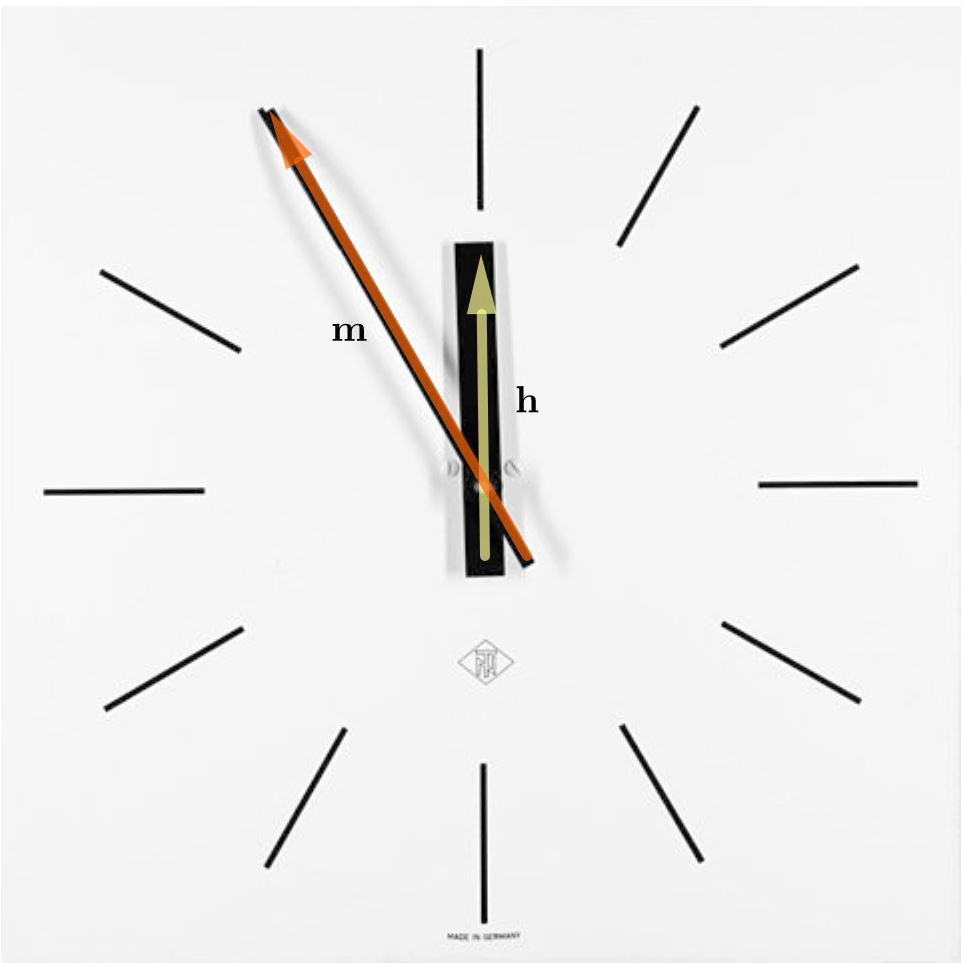
\includegraphics[height=2in]{clockvectors.jpg}
\end{center}

Answer:$$\vec{m}\dotp\vec{h}\text{ is greatest at }\answer{12}:00 \text{ o'clock}$$
$$\vec{m}\dotp\vec{h}\text{ is smallest at }\answer{6}:00 \text{ o'clock}$$
\end{problem}

\begin{problem} \label{prob:righttriangleincircle}
Let $O$ be a circle of radius $r$.  Suppose $A$ and $B$ are the endpoints of a diameter of $O$, and $C$ is a point on $O$ distinct from $A$ and $B$. Show that vectors $\overrightarrow{AC}$ and $\overrightarrow{BC}$ are orthogonal.  

\begin{hint}
Assign coordinates to points $A$, $B$ and $C$, express vectors $\overrightarrow{AC}$ and $\overrightarrow{BC}$ in component form, then find the dot product of $\overrightarrow{AC}$ and $\overrightarrow{BC}$.
\end{hint}

\begin{center}
\begin{tikzpicture}[scale=2]

  \draw[] (-1.3,0)--(1.3,0);
  \draw[] (0,-1.3)--(0,1.3);
   
\draw[](0,0) circle (1cm);

    \draw[line width=0.5pt,red](-1,0)--(0.5,0.87);
   \draw[line width=0.5pt,red](1,0)--(0.5,0.87);
   
   \fill[] (1,0)node[above right]{$B$} circle (0.05cm);
   \fill[] (-1,0)node[above left]{$A$} circle (0.05cm);
   \fill[] (0.5,0.87)node[above right]{$C$} circle (0.05cm);
 \end{tikzpicture}
\end{center}
\end{problem}

\begin{problem}\label{prob:rhombusdot} A rhombus is a quadrilateral with four congruent sides.  Use vectors to prove that a parallelogram is a rhombus if and only if its diagonals are perpendicular.
\begin{hint}
See section on vector subtraction in \href{https://ximera.osu.edu/linearalgebradzv3/LinearAlgebraInteractiveIntro/VEC-0030/main}{Vector Arithmetic}.
\end{hint}
\end{problem}

\begin{problem}\label{prob:pythagoreanR3usedotp}
 The points $A(2,1,4),B(4,2,-1)$, and $C(6,8,7)$ form a triangle in $\RR^3$.  Is it a right triangle?
\begin{hint}
Express each side of the triangle as a vector and use what you have learned in this section.
\end{hint}
\end{problem}

\section*{Photo Credits}
The following images are courtesy of \href{https://commons.wikimedia.org/wiki/Main_Page}
{Wikimedia Commons}

\noindent Hannes Grobe, \dfn{Wall clock manufactured by Telefonbau \& Normalzeit.} CC-BY 3.0



\end{document} 